\documentclass[12pt,twoside]{article}

% *** Set page dimensions ***
\raggedbottom
\parindent=0in
%\setlength{\topmargin}{-0.5in}
%\setlength{\oddsidemargin}{0.1875in}
%\setlength{\evensidemargin}{0in}
%\setlength{\textheight}{8.5in}
%\setlength{\textwidth}{6.225in}
%\addtolength{\oddsidemargin}{-0.7in}
%\addtolength{\evensidemargin}{-1.2in}
%\setlength{\oddsidemargin}{-0.2in}
%\setlength{\evensidemargin}{-0.2in}
%\addtolength{\textwidth}{1.4in}
%\addtolength{\topmargin}{-.875in}
%\addtolength{\textheight}{2.00in}

% *** Packages ***
\usepackage{alltt}
\usepackage{tocloft}
\usepackage{graphicx}
\usepackage{lscape}
\usepackage{amssymb}
\usepackage{float}
\usepackage{amsmath}
\usepackage{gensymb}
%\usepackage{subfigure}
\usepackage{lscape}
\usepackage{epsfig}
\usepackage{enumerate}
\usepackage{multicol}
\usepackage{fancyhdr}
\usepackage{epstopdf}
\usepackage{hyperref}
\usepackage{listings}

% *** Table of contents and Sectioning *** 
\setcounter{secnumdepth}{0}
\setcounter{tocdepth}{5}

% *** Table of contents and Sectioning *** 
\newcommand{\next}{\addtocounter{enumi}{9} \item}
\newcommand{\now}[1]{\setcounter{enumi}{#1}}
\newcommand{\Z}{\mbox{\sf Z\hspace{-1.5mm}Z}}
\newcommand{\R}{\mbox{\rm I\hspace{-0.75mm}R}}
\columnsep=0.75in

% *** Shortcuts for syntax ***
\newcommand{\ds}{\displaystyle }
\newcommand{\vsc}{\vspace{4mm}}
\newcommand{\dd}[1]{\frac{d}{d{#1}} \,} 
\newcommand{\ddx}{\frac{d}{dx} \,} 
\newcommand{\ddy}{\frac{d}{dy} \,} 
\newcommand{\ddz}{\frac{d}{dz} \,} 
\newcommand{\dydx}{\frac{dy}{dx} \,} 
\newcommand{\dydt}{\frac{dy}{dt} \,} 
\newcommand{\dfdx}{\frac{df}{dx} \,} 
\newcommand{\ddt}[1]{  \frac{d{#1}}{dt} }
\newcommand{\pp}[2]{  \frac{\partial{#1}}{\partial {#2}} }
\newcommand{\zx}{\frac{\partial z}{\partial x} \,}
\newcommand{\zy}{\frac{\partial z}{\partial y} \,}
\newcommand{\limh}{\lim_{h \rightarrow 0} \;}
\newcommand{\diff}{\frac{d}{dx} \,}
\newcommand{\de}{\Delta}
\renewcommand{\thesection}{\Roman{section}}
\newcommand{\bfr}{\begin{flushright}}
\newcommand{\efr}{\end{flushright}}
\newcommand{\dx}{\frac{\partial f}{\partial x} \,}
\newcommand{\dy}{\frac{\partial f}{\partial y} \,}
\newcommand{\p}{\partial}
\newcommand{\vi}{\vec{i}}
\newcommand{\vj}{\vec{j}}
\newcommand{\vk}{\vec{k}}
\newcommand{\lan}{\left\langle}
\newcommand{\ran}{\right\rangle}
\newcommand{\reading}[1] { {\em Reading: #1}}
\renewcommand{\Pr}{ \mbox{Pr}}

% *** Commands related to textbook references
\newcommand{\problem}{{\bf Problem.} }

% *** Footnoting with symbols ***
\long\def\symbolfootnote[#1]#2{\begingroup%
\def\thefootnote{\fnsymbol{footnote}}\footnote[#1]{#2}\endgroup}

% *** Defining a boxed note ***
\floatstyle{boxed}
\newfloat{noteinbox}{htb}{loa}
\newenvironment{boxnote}{\begin{noteinbox}[H]}{\end{noteinbox}}

\newcommand{\Question}{ {\bf Question: }  }
\newcommand{\Example}[1]{ {\bf Example: } {\em #1} }
\newcommand{\ExampleCont}[1]{ {\em #1} }

% *** Define the boxed Week #/summary at the beginning/end of every chapter ***
\newcommand{\sectionbox}[1]{% 
\begin{tabular}{|p{6in}|}%
\hline%
\ \\ %
{\Large {\bf {#1}}}  \\%
\ \\%
\hline%
\end{tabular}}

% *** Shortcuts *** 
\newcommand\goals{\large {\bf {Goals:}}}
\newcommand\setfont{ }

% *** Week commands: overwritten in each notes file
\newcommand{\Week}{Null-InPreambleCommon}
\newcommand{\WeekTitle}{Null-InPreambleCommon}
\newcommand{\Course}{MNTC P04}
\newcommand{\SetNum}{1 }
\newcommand{\topic}[1]{
\newpage
\setcounter{page}{1}
\fancyhead[LE,RO]{#1 - \thepage}
}

% *** Setup Latex for the large version of the files ***
%\usepackage[landscape]{geometry}
\usepackage[letterpaper,landscape,hmargin={.8in,.8in},vmargin={1in,0.2in}]{geometry}

% Remove paragraph indents
\setlength{\parindent}{0pt}

% Spacing at the top for the header is too large by default
\setlength{\voffset}{-5ex}

% **** RENEW SCALING COMMANDS HERE ****
% *** Text in boxes ***
\renewenvironment{boxnote}{\begin{noteinbox}[H] \huge}{\end{noteinbox}} 

% *** Chapter lead in/summary boxes ***
\renewcommand{\sectionbox}[1]{% 
\begin{tabular}{|p{9.5in}|}%
\hline%
\ \\ %
{\huge {\bf {#1}}}  \\%
\ \\%
\hline%
\end{tabular}}

% *** 'Section'' commands, which are sometimes used for spacing
% From http://zoonek.free.fr/LaTeX/LaTeX_samples_section/0.html
\makeatletter
 \renewcommand\section{\@startsection {section}{1}{\z@}%
                                    {-3.5ex \@plus -1ex \@minus -.2ex}%
                                    {0.3ex \@plus.2ex}%
                                    {\setfont\bf}}

 \renewcommand\subsection{\@startsection {subsection}{1}{\z@}%
                                    {-3.5ex \@plus -1ex \@minus -.2ex}%
                                    {0.3ex \@plus.2ex}%
                                    {\setfont\bf}}

% *** 'Goals' should be larger in the overheads ***
\renewcommand\goals{\huge {\bf {Goals:}}}
\renewcommand\setfont{\huge }

\thispagestyle{empty}

\setfont 

\newcommand{\WeekTitleOne}{Derivatives - Foundations}
\newcommand{\WeekTitleTwo}{Derivatives - Linearization and Applications}
\newcommand{\WeekTitleThree}{Derivatives - Modeling}
\newcommand{\WeekTitleFour}{Integrals - Foundations}
\newcommand{\WeekTitleFive}{Integrals - Techniques}
\newcommand{\WeekTitleSix}{Integrals - Modeling}
\newcommand{\WeekTitleSeven}{Differential Equations - }
\newcommand{\WeekTitleEight}{Differential Equations - }
\newcommand{\WeekTitleNine}{Differential Equations - }
\newcommand{\WeekTitleTen}{Linear Algebra - }
\newcommand{\WeekTitleEleven}{Linear Algebra - }
\newcommand{\WeekTitleTwelve}{Linear Algebra - }



\begin{document}
\setfont
\pagestyle{fancy}
\renewcommand{\Week}{9 }
\renewcommand{\WeekTitle}{\WeekTitleNine }

\fancyhead[LE,RO]{Week \Week}  % default, usually only for first page
\fancyfoot{}
\sectionbox{Week \#\Week: \WeekTitle}


\vspace{5mm}
\goals
\begin{itemize}
\item Take problems that can be modeled by differential equations,
  both first and second order, and give solutions both by hand and
  MATLAB (CLO5, CLO8)
\item Examine case studies of differential equations applied to
  engineering problems and reproduce those solutions
\end{itemize}
\vspace{5mm}

\newpage

\subsection*{Example - Pendulum }
\vfill
\begin{align*}
  \mbox{Newton's Second Law: }   m  L^2 \theta'' & = T_g + T_f  \\
  & = - m L g \sin(\theta) - (\mu L^2 m) \theta' \\
  \mbox{Solving for $\theta''$: }\theta'' & = - \frac{g}{L} \sin(\theta) - \mu 
  \theta'
\end{align*}

\problem Turn this single second-order DE into a pair of first-order
DEs.

\newpage


\problem Download the representation of this system of DEs,
  \texttt{pendulumDE.m}.  Compare it to our DE system,
\begin{align*}
\frac{d y_1}{dt} & = y_2 \\
\frac{d y_2}{dt} & = -\frac{g}{L}\sin(y_1)  - \mu y_2
\end{align*}
\vsc

\problem Download and run the script \texttt{W8\_2.m}.

\vsc

\problem What were the initial conditions of the pendulum?

\vfill

\problem Based on that information, what do the two curves on the graph
  represent?

\vfill

\newpage

\problem Change the script so the pendulum also has an initial velocity.

\vsc

\problem If we keep the initial angle at $-\frac{\pi}{2}$ (pendulum
  out horizontally), experiment and find the initial velocity that
  will push the pendulum ``over the top''.

\topic{Deformation of a Loaded Beam}
\section*{Deformation of a Loaded Beam} 
~\\[1ex]

\begin{minipage}{3.2in}
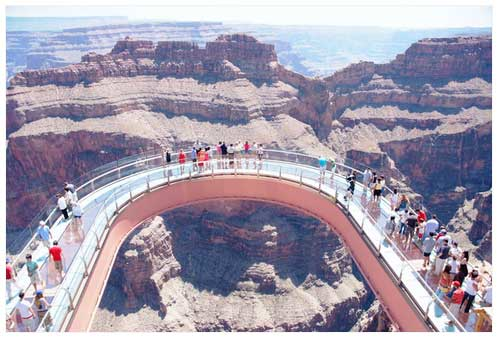
\includegraphics[width=3in]{graphics/notes_09_GrandCanyonWalkway} \\
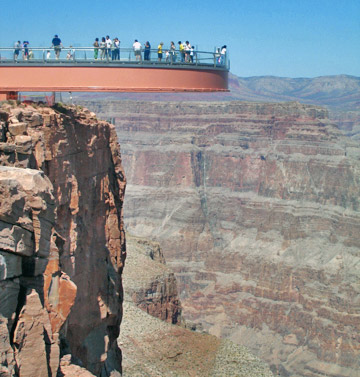
\includegraphics[width=3in]{graphics/notes_09_GrandCanyon_SkywalkFromOutsideLedge}
\end{minipage}
\begin{minipage}{4in}
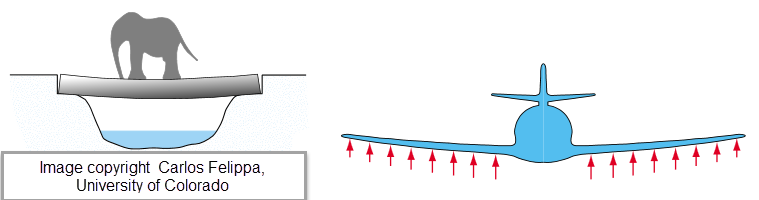
\includegraphics[width=7in]{graphics/notes_09_BeamExamples_CarlosFelippa} \\
\end{minipage}

\newpage

The physics of how beams deform isn't central to this course, and
engineering students in particular will take a course on structures
that goes into deeper detail.  For our purposes, it is enough to be
able to use the resulting differential equations.

$$EI y^{(4)} = p(x)$$
where  \\
$y(x)$ is the deflection (distance away from a straight line),  \\
$p(x)$ is the loading in N/m at point $x$ along the beam, \\
$E$ is a value related to the material of the beam, and  \\
$I$ is a value derived from the cross-sectional size and shape of the
beam.

\newpage
\problem
  Find the form of $y_c$ for the beam deflection DE, assuming $E$ and
  $I$ are constant.
$$EI y^{(4)} = p(x)$$

 \newpage


\topic{Cantilevered Beam Under Uniform Load} 
\subsection*{Cantilevered Beam Under Uniform Load} 

 Under a uniform loading (constant force per unit length), a {\em
   cantilevered beam} which is $L = 2$ m long, made out of a pine ``2 by 4'' satisfies \\
 $p(x) = 100$ N/m, (or roughly 10 kg applied to each meter) \\
 $I = 2.23 \times 10^{-6}$ m$^4$,\hspace{0.5in} $E = 9.1 \times
 10^{9}$ N/m$^2$,
 
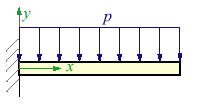
\includegraphics[width=3in]{graphics/notes_09_CantileveredBeam_Diagram}

and the {\em boundary} conditions 
$y(0) = 0$, $y'(0) = 0$, $y''(2) = 0$, and $y'''(2) = 0$.

\problem
  Find the amount of deflection of the beam at the tip under this
  load.

\newpage
\hfill $EI y^{(4)} = 100$
 
~\hfill
$y(0) = 0$, $y'(0) = 0$, 

~\hfill $y''(2) = 0$, and $y'''(2) = 0$.

\newpage
\problem
  If the maximum allowable deflection in such a beam is only 0.2 cm
  (say in a building code), what would the maximum uniform load be?
\end{document}
%Confirmation of deflection:
%  http://www.efunda.com/formulae/solid_mechanics/beams/casestudy_display.cfm?case=cantilever_uniformload


\end{document}

